\documentclass[border=5mm,tikz]{standalone} 

\usepackage{amsmath}
% !TEX root=img/arguments_and_attack.tex

% \usetikzlibrary{external} 
% \tikzexternalize[prefix=tikz/] 

\usetikzlibrary{calc}
\usetikzlibrary{arrows}
\usetikzlibrary{arrows.meta}
\usetikzlibrary{decorations.markings}
% \usetikzlibrary{intersections}
\usetikzlibrary{fit}
\usetikzlibrary{shapes}
% \usetikzlibrary{trees}


\tikzset{
	every path/.style={thick},
	align=center,
	observed/.style={
		fill=black!20,
	},
	bn/.style={
		draw,
		ellipse,
		-{Triangle[angle=60:6pt 0]}
	},
	scn/.style={
		draw,
		rectangle,
		% signal,
		% signal from=west,
		% signal pointer angle=120,
		-{Triangle[angle=60:6pt 0]},
	},
	possibly/.style={dashed},
	arg/.style={
		draw,
		rectangle,
		-{Straight Barb[angle=60:6pt 0]}
	},
	attack/.style={
		-{Rays[width=10pt,length=10pt,sep=-3.9pt]}
	},
	pref/.style={
		draw,
		rectangle,
		-{Straight Barb[angle=60:6pt 0]}
	},
	subscn/.style={
		double,
		-{Triangle[angle=60:6pt 0]},
	},
	specific/.style={
		double,
		-{Stealth[angle=60:6pt 0]}
	},
}



\begin{document}
	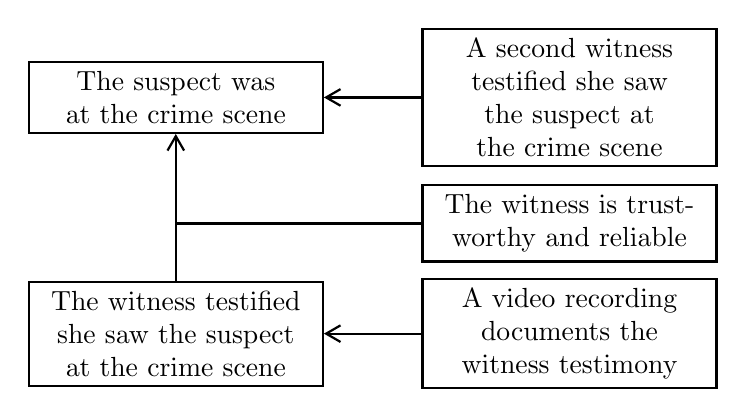
\begin{tikzpicture}[
		scnnode/.append style={text width=3cm},
		arg/.append style={text width=3.5cm},
	]
		\pgftransformxscale{5}
		\pgftransformyscale{2}

		\node[arg]     			(scene) at (0,-0.5) {The suspect was at the crime scene};
		\node[arg] 					(witn) at (0,-2) {The witness testified she saw the suspect at the crime scene};

		\node[arg] 					(alibi) at (1,-0.5) {A second witness testified she saw the suspect at the crime scene};
		\node[arg] 					(lying) at (1,-1.3) {The witness is trustworthy and reliable};
		\node[arg] 					(fraud) at (1,-2) {A video recording documents the witness testimony};

		\draw[arg] 					(witn) -- (scene);

		\draw[arg] 			(alibi) -- (scene);
		\draw 					(lying) -- (0, -1.3);
		\draw[arg] 			(fraud) -- (witn);

%%%

		%\node[arg]     			(scene) at (1.85,-0.5) {The suspect was at the crime scene};
		%\node[arg] 					(witn) at (1.85,-2) {The witness reports that she saw the suspect at the crime scene};
%
		%\node[arg] 					(lying) at (2.35,-1.15) {The witness report is trustworthy};
%
		%\draw[arg] 					(witn) -- (scene);
%
		%\draw 					(lying) -- (1.85, -1.15);




	\end{tikzpicture}
\end{document}
